\section{Introduction}
\label{sec:intro}



Counterfactual reasoning --- mentally simulating what \emph{would have happened} if conditions were different --- is a common tool for making causality assessments~\cite{kahneman}, which in turn are crucial for model training, evaluation, and explanation~\cite{miller}. 
For example, in Figure~\ref{fig:teaser}, \exinline{It is great for kids} is perturbed into multiple variations, each providing unique insights by simulating what would have happened if the sentence was different.


%\hao{suggestion: it could be great if you can highlight the high cost of existing approaches by being more specific on, \eg the cost of human annotation and cite some works backing it up. something like the human annotation in xxx costs xxx money/time would be very convincing. }
Applications of counterfactual reasoning to NLP generally specify the relationship $x \veryshortarrow \xp$, and then create $\xp$ according to the relationship.
As a result, prior work has tailored counterfactual generators for every application, which induces different limitations.
%For example, a minimal edit of a sentence $x$ that results in a different label is useful for model training and evaluation.
%Such counterfactuals are usually produced manually by human annotators ~\cite{gardner2020contrast} or by human-written perturbation functions~\cite{wu2019errudite}, making them costly to generate (\eg 4-5 minutes per counterfactual \cite{kaushik2019learning}) and liable to systematic omissions (\eg human annotators may miss \swap{kids}{no one} in Figure \ref{fig:teaser}B). %Further, relying on human creativity may cause important but non-obvious patterns to be missed, \eg humans may cover \swap{great}{not great}, but miss \swap{kids}{no one} in Figure~\ref{fig:teaser}B.
%Though it is cheaper to automate the process with parsing templates~\cite{li2020linguistically}, the templates usually have limited coverage on either the patterns-to-perturb, or the applicable data points.
%In contrast, adversarial examples specify a very different counterfactual relationship: $x$ and $\xp$ must have different model predictions \emph{despite} being semantically equivalent, such that automated methods often rely on paraphrasing models~\cite{iyyer2018adversarial, ribeiro2018semantically}.
For example, to support model training and evaluation, human annotators collect counterfactuals that change the groundtruth labels by manually rewriting instances~\cite{gardner2020contrast} or defining perturbation functions~\cite{wu2019errudite}.
The manual rewrites are costly (\eg 4-5 minutes per counterfactual \cite{kaushik2019learning}) and liable to systematic omissions (\eg human annotators may miss \swap{kids}{no one} in Figure \ref{fig:teaser}B).
The focus on label-flipping relationships also largely ignores the benefit from label-preserving ones on model robustness.
In contrast, adversarial examples specify a different relationship: $x$ and $\xp$ must have the same groundtruth but different model predictions, driving the generator to prioritize straightforward paraphrasing or synonym replacement~\cite{iyyer2018adversarial, ribeiro2018semantically}, over alternatives that change the semantic meaning (\eg negating sentences in named entity recognition).

\begin{figure}[t]
\centering
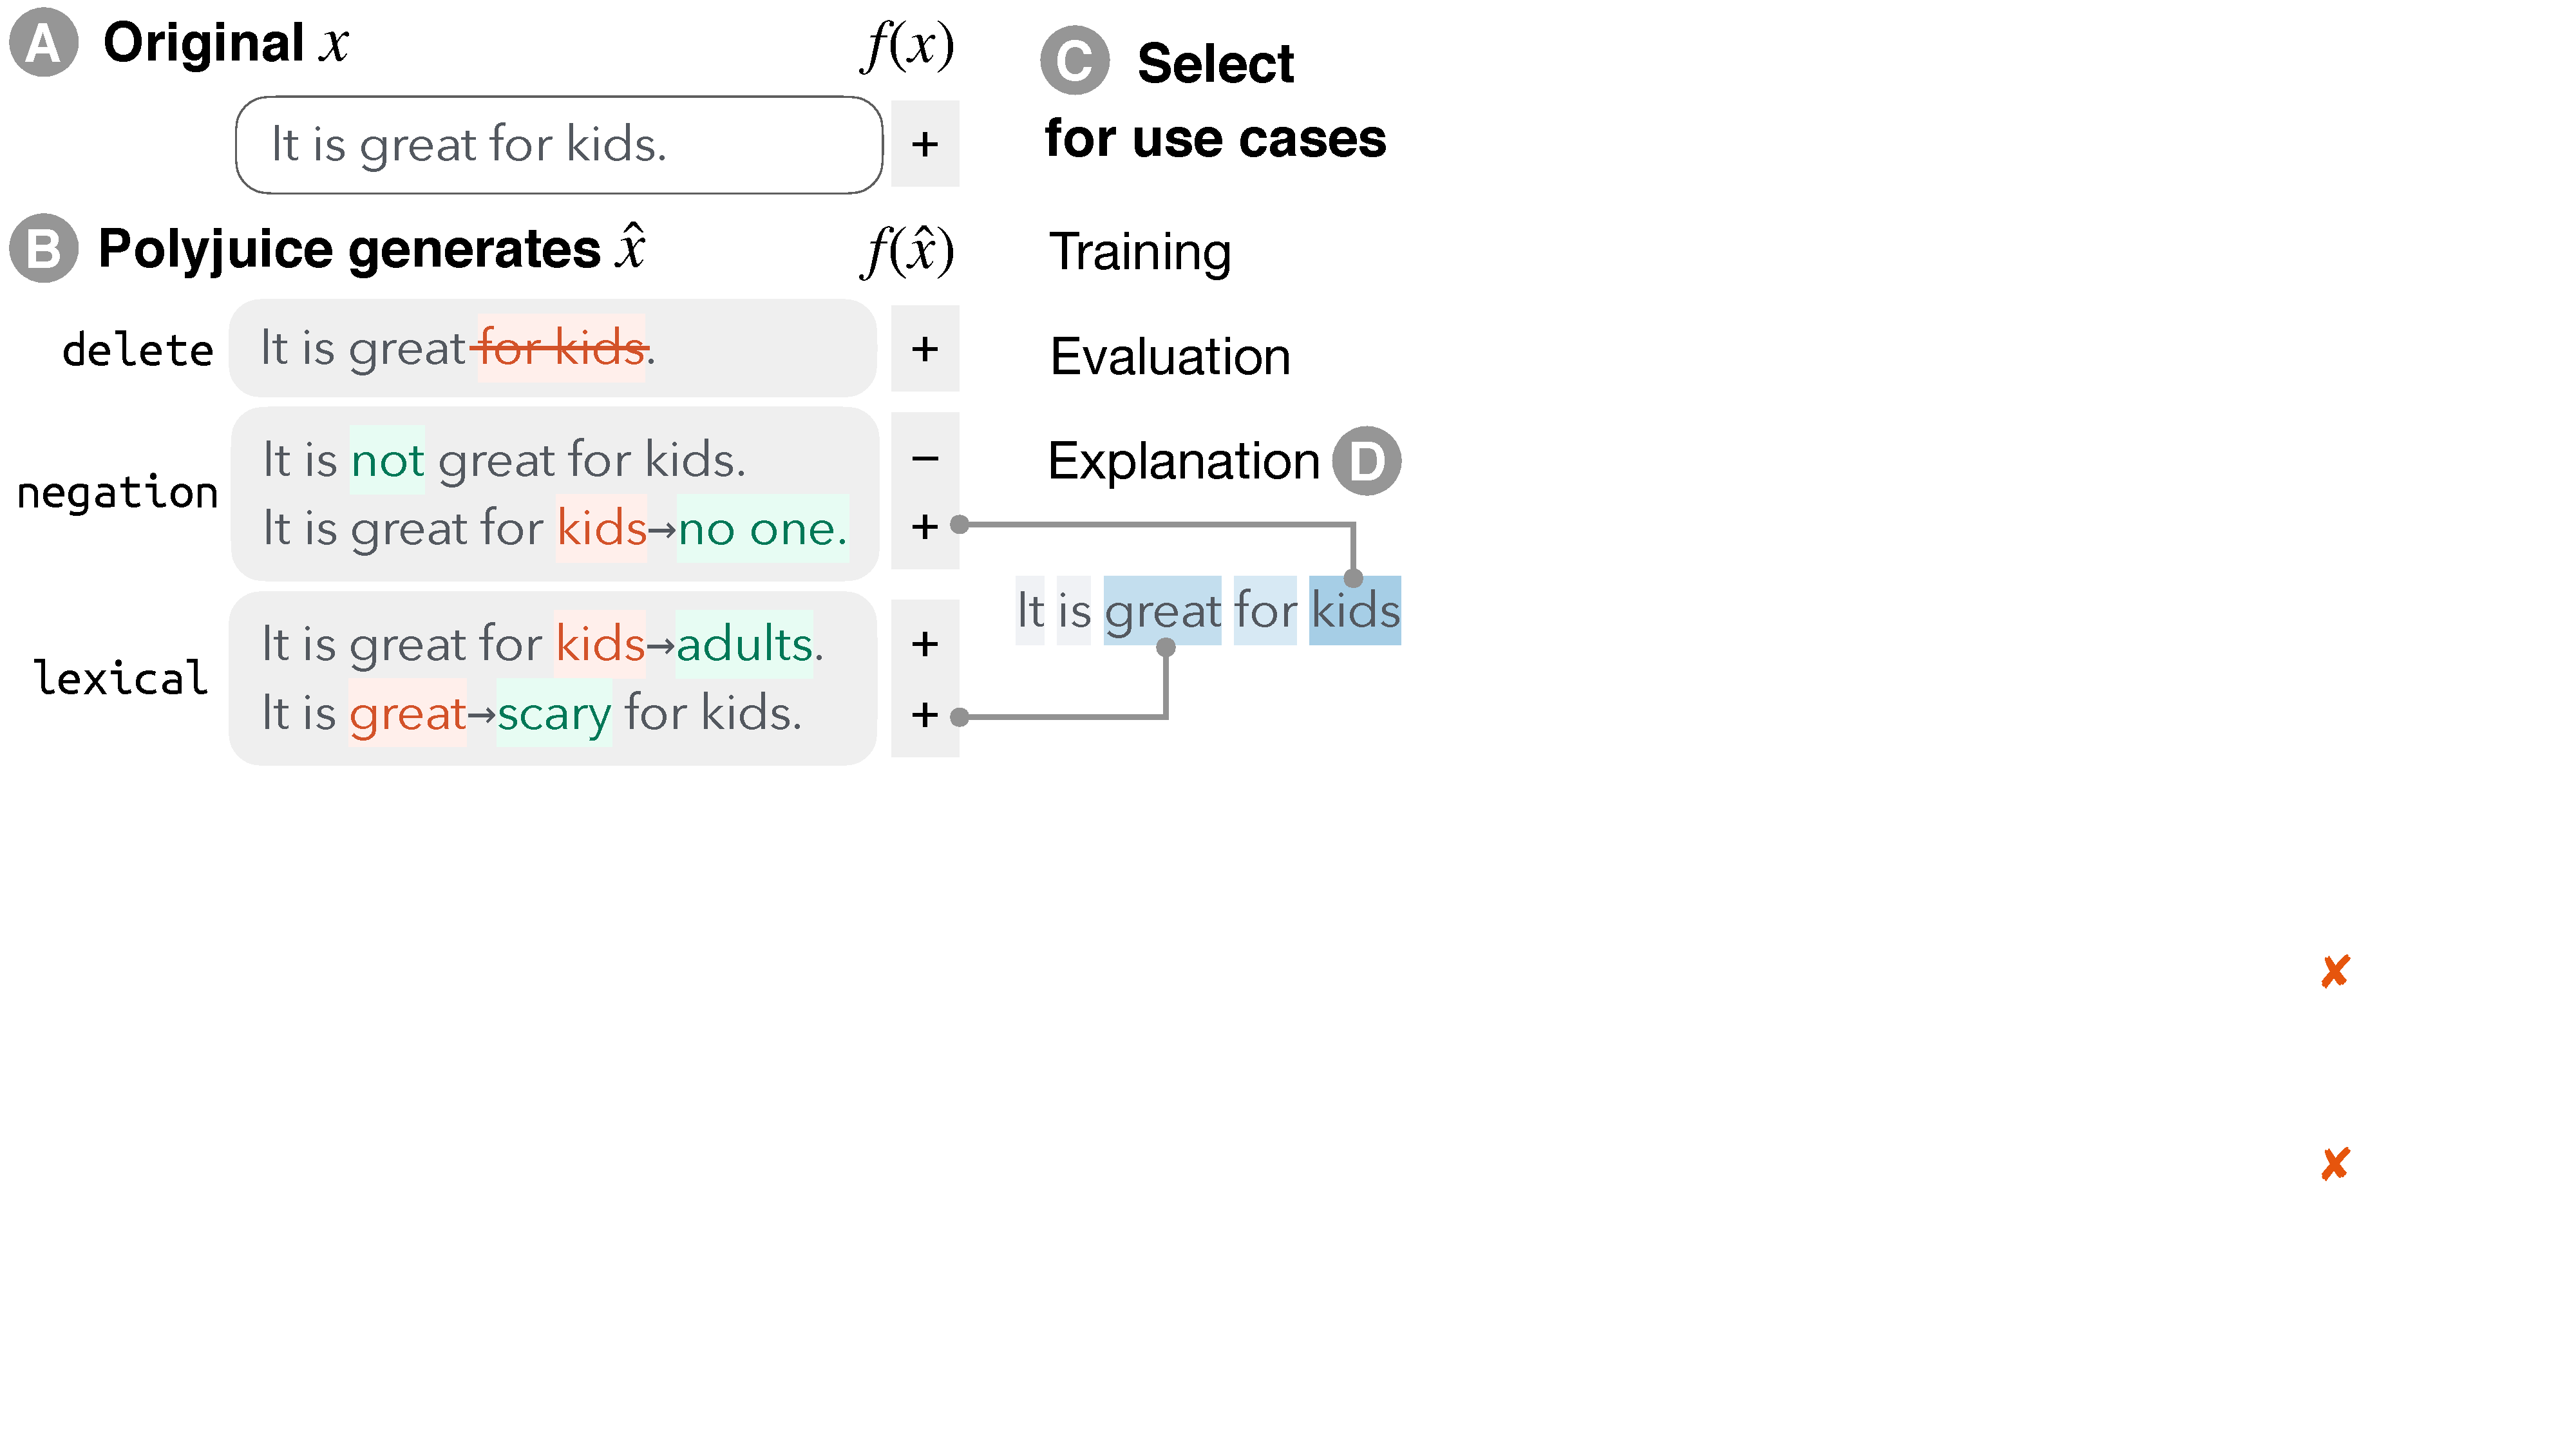
\includegraphics[trim={0 18cm 30.5cm 0cm},clip, width=1\columnwidth]{figures/teaser.pdf}
\vspace{-15pt}
\caption{
Overview: (A) given sentiment analysis instance $x$, \sysname generates (B) a large set of perturbations $\xp$, which are then (C) selected for downstream use.
For example, in (D) we select counterfactual explanations that complement the feature attributions: though both ``great'' and ``kids'' are deemed important, perturbing them may not affect the prediction $f(x)=f(\xp)=\text{\emph{positive}}$, revealing model errors.\footnotemark
}
\vspace{-15pt}
\label{fig:teaser}
\end{figure} 
\footnotetext{We opensource both the \sysname model and the selection strategies at \modelurl.}


%However, as Figure \ref{fig:teaser} illustrates, counterfactual generation does not \emph{have} to be task-specific, as various applications share similar requirements on $x\veryshortarrow\xp$ (\eg a preference for small changes).
%In fact, a general-purpose pool of diverse counterfactuals may be preferable when the relationship is not precisely defined in advance, as is the case for counterfactual training, evaluation, or explanations.
% In fact, a common pool of counterfactuals may support each application more comprehensively.
% For example, without the preset constrain on semantic equivalence, we can collect adversarials through negation (for tasks insensitive to negation, \eg named entity recognition.)
%For example, some forms  in training and evaluation data collection can 
%The exhaustive search of automated methods can cover the training and evaluation more comprehensively, and non-paraphrasing changes like \emph{add negation} are valuable adversarials for tasks like named entity recognition. 
%\hao{might be good to clarify that these two are not mutually-exclusive: adversarial examples should sometimes be close to the original}
% 
However, counterfactual generation does not \emph{have} to be task-specific.
As shown in Figure~\ref{fig:teaser}, the same set of counterfactuals can be useful for a variety of applications.
Moreover, in open-ended uses cases like counterfactual explanation (Figure~\ref{fig:teaser}D) and analysis, a general-purpose pool of diverse counterfactuals is preferable, as the relationship is not precisely defined in advance.
In this work, we formalize the task of \emph{automatic counterfactual generation}, which disentangles generation from the application of counterfactuals.
Given an input $x$, our generator produces a set of counterfactuals $\hat{\xset} = \{\xp_1, \xp_2, ...\}$ with reasonable but \emph{application-agnostic} relationships $x \veryshortarrow \xp_i$ (Figure~\ref{fig:teaser}B).
We require counterfactuals to be \emph{fluent}, \emph{diverse}, and \emph{close to $x$}.
Afterwards, we use \emph{application-specific} selection methods to find subsets of $\xp$ that are most effective for the application of interest (Figure~\ref{fig:teaser}C).
We frame the generation step as conditional text generation, and finetune GPT-2~\cite{radford2019language} into a generator called \emph{\sysname} using datasets of $(x, \xp)$ pairs. 
We also allow for targeted counterfactuals, by specifying where the perturbation occurs in the sentence~\cite{donahue2020enabling} and using \tagstrs such as \ctrltag{negation} or \ctrltag{delete} (Figure~\ref{fig:teaser}B).
%--- the control is \emph{the backbone of} various downstream applications.

We propose simple yet effective selection strategies, and show that a single \sysname model can significantly aid humans in diverse downstream applications. For \emph{counterfactual training and evaluation}, humans label \sysname counterfactuals rather than creating them from scratch, resulting in training data that significantly improves model generalization, as well as high-quality contrast sets~\cite{gardner2020contrast}, with 40--75\% less annotation effort ~\cite{kaushik2019learning}. In another application, \sysname produces \emph{counterfactual explanations} that bring significant insights that extend beyond state-of-the-art explanation techniques. Finally, \sysname supports counterfactual \emph{error analysis} by allowing users to explore related counterfactuals (\eg the model responds differently to different negation forms in Figure \ref{fig:teaser}B) and to aggregate individual counterfactuals into patterns in order to systematically understand model behavior.

%First, 
% By lifting the burden of manual rewrite, \sysname \emph{facilitates effective counterfactual training and evaluation}.
% With humans only \emph{labeling} counterfactuals, we produce training data that improves model generalization, as well as high-quality contrast sets~\cite{gardner2020contrast} with 40\%--75\% less annotation effort compared to creating them from scratch~\cite{kaushik2019learning}. 
%We similarly produce training data that improves model generalization in three classification tasks. %, when compared to adding the same amount of non-counterfactual data.

% (2) 
% %Second, 
% By generating nontrivial counterfactuals beyond paraphrasing and human intuitions, \sysname helps \emph{produce counterfactual explanations} that highlight model errors obscure to humans. 
% In a user study, experts only did slightly better than random (accuracy: $55 \pm 6\%$) at predicting what a model would do on \sysname counterfactuals, even after inspecting the model on their own.
% (3) 
% %Third, 
% By rewriting each instance in multiple ways, \sysname \emph{supports more systematic error analysis}.
% Case studies demonstrate that \sysname counterfactuals help contrast model behaviors on related perturbations (\eg the model in Figure~\ref{fig:teaser} responds differently to the two negation forms.)

% We opensource both the \sysname model and the selection strategies at \modelurl.


\begin{comment}
In summary, we:
\begin{compactenum}
\item  Formalize the general-purpose counterfactual generation task. 
By \emph{separating the generation from the use cases}, we generate fluent and diverse counterfactuals that bypass application-specific constraints.
%. \hao{maybe emphasize the benefits of this}
\item Finetune a generator called \sysname, by collecting paired sentences and enhancing controls with infilling structures and \tagstrs --- the control is \emph{the backbone of} various downstream applications.
%\sysname generates plausible and diverse counterfactuals, with control over where perturbations happen and what they do.
The model is at \modelurl.
%, and we plan to opensource the selection strategies.
\item Apply \sysname to \emph{model training, evaluation, and explanation}, using various selection methods (which we will opensource).
\sysname helps collect high-quality training and evaluation data with 40\% less annotation effort, and find model bugs that on top of feature attribution explanations and counterfactual analysis.
\end{compactenum}
\wts{Maybe can delete if we run out of space.}
\end{comment}

% we observe that \sysname explanations can complement popular feature attribution methods and highlight their blind spots.
% After viewing SHAP weights~\cite{NIPS2017_7062} and interacting with the model, experts still could not predict model behaviors on counterfactuals selected for explanations, and missed 5\% and 25\% more cases than the human-generated or random baselines.
